\documentclass[11pt]{article}

\newcommand{\thetitle}{Memo: Testing Horn Signal Chain Power Levels}
\newcommand{\theauthor}{Kara Kundert}
\newcommand{\theauthorsemail}{kkundert@berkeley.edu}
\newcommand{\thedate}{\today}
% the following controls some aspects of how the text is displayed on the page
\setlength{\textwidth}{6.5in}
\setlength{\textheight}{8.25in}
\setlength{\oddsidemargin}{0in}

% set up the page headers and footers
\usepackage{fancyhdr}
    \pagestyle{fancy}
    \lhead{\sffamily\slshape\small\thetitle}
    \rhead{\sffamily\small\theauthor}
    \cfoot{\sffamily\slshape\small\thepage}

\usepackage{graphicx} % support display of graphics
\usepackage{amsmath,amssymb,latexsym} % import library of technical symbols

% the following control some aspects of how paragraphs are displayed
\parindent=0pt
\parskip=2ex

\begin{document}
% print the title in san-serif font, in bold, in huge characters
\title{
    \sffamily\bfseries\huge
    \thetitle \\
}
% print the author in san-serif font
\author{
    \sffamily\theauthor \\
    \sffamily\theauthorsemail
}
\date{\centering\thedate}
\maketitle
\sloppy

\begin{abstract}
 In order to ease future understanding and debugging of issues with the horn 
 signal chain, we have generated this report inputting a known test tone and 
 noise into the signal chain. We have then followed its evolution as it moves 
 through the signal chain, verified power levels and frequency shifts, so that 
 future users may be better able to track down faults quickly.
\end{abstract}

\section{Introduction}

The basic layout of the signal chain is this: it takes a low power 1.4GHz 
signal incoming from the horn, filters and amplifies and downconverts it, 
enabling us to sample it adequately and do astronomy with the data. A full 
signal chain is shown in Fig.~\ref{fig:block-diagram}. In order to be able to 
collect reasonable data, two key things must be true of the signal chain:

\begin{figure}
    \begin{center}
    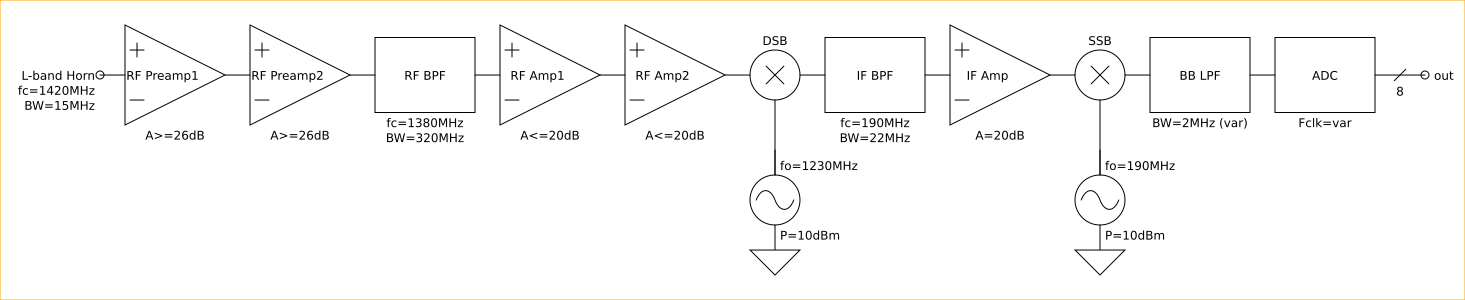
\includegraphics[width=\linewidth]{block_diagram.png}
    \end{center}
    \caption{
        The full horn signal chain from the L-band horn to the PicoScope 2000 
        digital sampler. Note that the second pair of RF amplifiers has a gain 
        specification of 20 dB each, but the combined gain output is only about 
        $A_{total} \approx 30$ dB in reality.
    }
    \label{fig:block-diagram}
\end{figure}

\begin{enumerate}
 \item The mixers must be shifting the frequencies of the signal in the way we 
  expect, such that the band that we do end up sampling is the one that 
  contains the 21cm signal from the horn.
 \item The amplifiers must be providing enough gain in order to toggle enough 
  bits in the ADC that we can actually see it, while also not generating strong 
  reflections that overwhelm the system.
\end{enumerate}

So let us first figure out how much power we need at the ADC. Let's say we want 
a 100 mV signal incoming to the ADC. Using Ohm's Law, a 100 mV signal would 
generate $P_{mW} = 0.04$ mW. Now, using Eq.~\eqref{eq:dBm}, we can convert that 
into $P_{dBm} = -14$ dBm at the picosampler.

\begin{equation}
    \label{eq:dBm}
    P_{dBm} = 10 \log_{10}\Big(\frac{P_{mW}}{1~\textrm{mW}}\Big)
\end{equation}

\section{Method}

The average power from incoming from the horn is about $P = -58$ dBm. We 
attempted to construct a similar signal within the lab using a noise source and 
a signal generator. The NOD5250 noise generator was set to maximum attenuation 
(i.e. attenuator = 10), and was measured to be outputting broadband noise 
around $P = -47$ dBm. We wanted the tone to be small but trackable, so that was 
set at $\nu = 1421$ MHz and $P = -40$ dBm. These were combined using a 
backwards splitter, and the power levels were verified using a spectrum 
analyzer. Post-cabling and combination, the tone had a power level of 
approximately $P = -43$ dBm.

From here, we measured the power at multiple points within the signal chain.  
The results of these measurements are shown in Table~\ref{tab:power-levels}.

\section{Results}

All measurements are taken at the output of the given location.

\begin{center}
    \begin{tabular}{ c | c | c }
        \label{tab:power-levels}
        \textbf{Sample Location} & \textbf{Power Level} & \textbf{Tone 
        Frequency} \\
        \hline
        First Bandpass Filter & -45 dBm & 1421 MHz \\
        \hline
        Back-to-Back Amplifiers & -9 dBm & 1421 MHz \\
        \hline
        DSB Mixer & -16 dBm & 191 MHz \\
        \hline
        Second Bandpass Filter & -17.5 dBm & 191 MHz \\
        \hline
        Amplifier & 3 dBm & 191 MHz \\
        \hline
        SSB Mixer (Variable Filter Input 1) & -10 dBm & 1 MHz \\
        \hline
        SSB Mixer (Variable Filter Input 2) & -10 dBm & 1 MHz \\
        \hline
        Variable Filter (Output 1) & -14 dBm & 1 MHz \\
        \hline
        Variable Filter (Output 2) & -12 dBm & 1 MHz \\
    \end{tabular}
\end{center}

\end{document}
